\documentclass{article}
\usepackage{amsmath}
\usepackage{amssymb}
\usepackage[margin=1in]{geometry}
\usepackage{booktabs}
\usepackage{float}
\usepackage{graphicx}
\usepackage{hyperref}
\usepackage{pdfpages}

\title{Final Project\\Numerical Solutions to PDEs}
\date{9 May 2025}
\author{Connor Emmons and Noah Wells}

\begin{document}
\pagenumbering{gobble}
\maketitle
\begin{figure}[h]
    \centering
    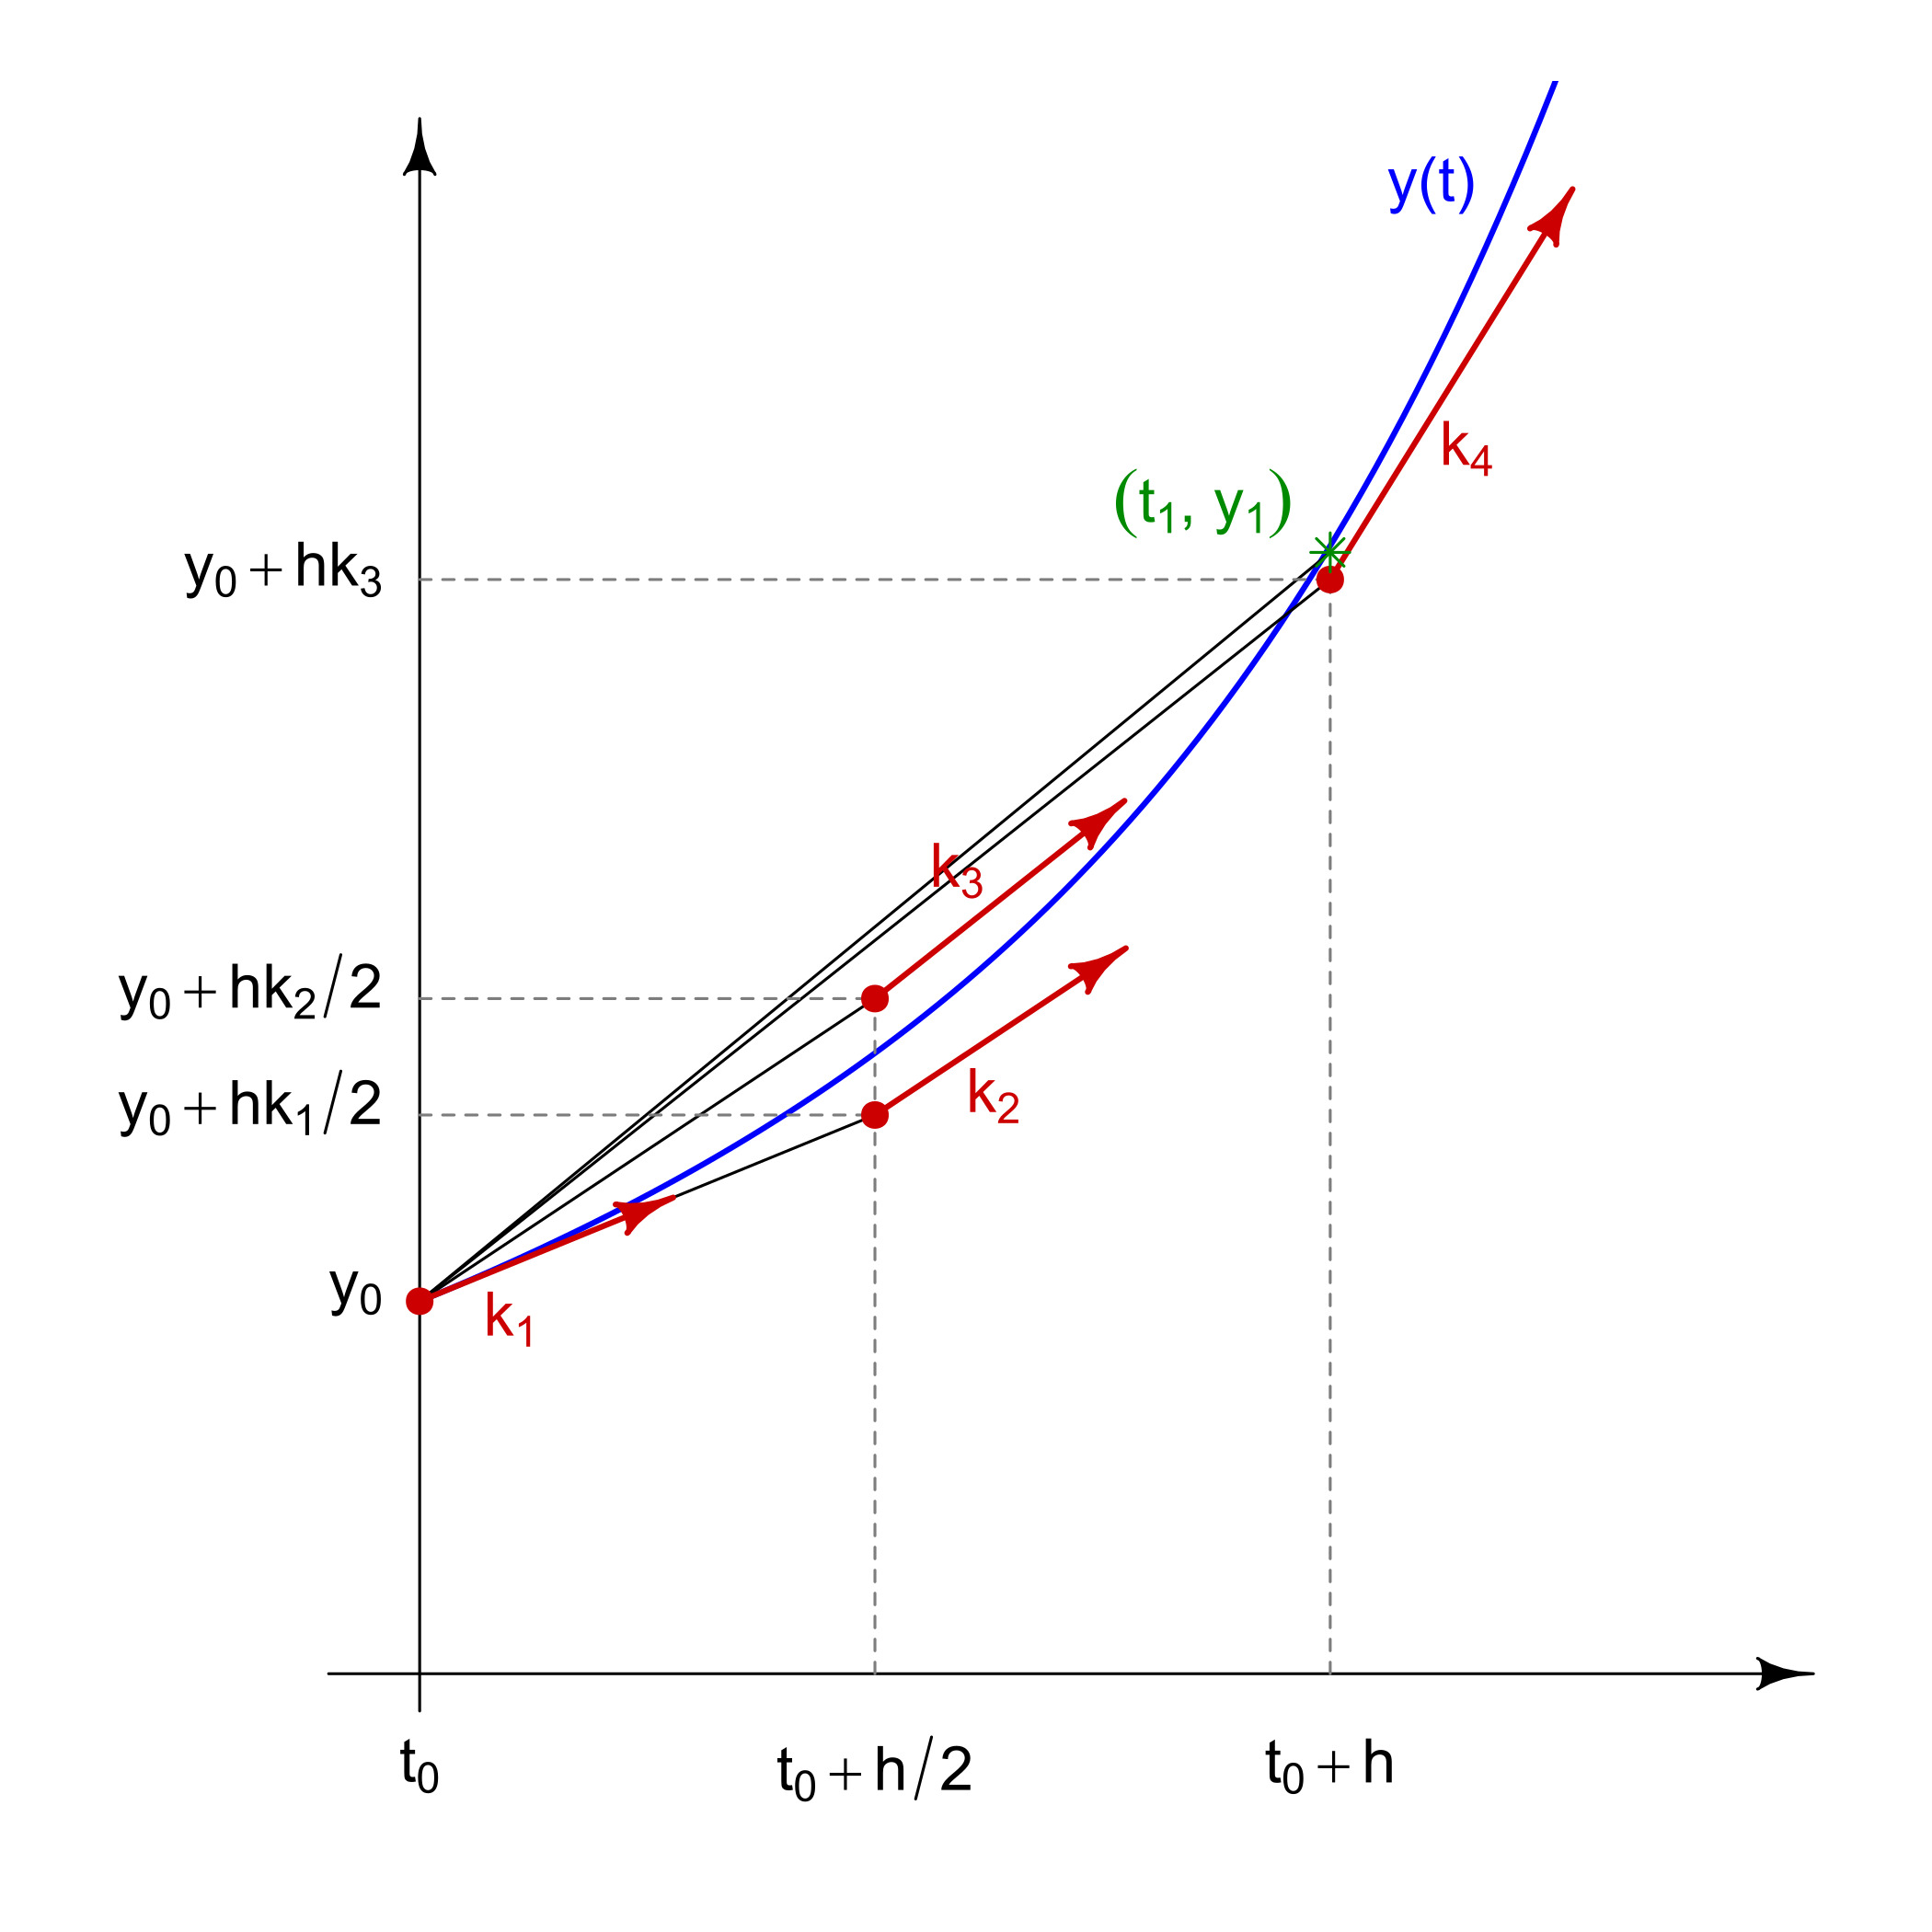
\includegraphics[width=0.8\textwidth]{title.jpg}
\end{figure}
\vfill
\paragraph*{Documentation}
UPDATE THIS
\newpage
\pagenumbering{arabic}

\section{Basic Heat Equation}

\subsection*{$u_t = 2u_{xx}\\u(0,t) = u(3,t) = 0\\u(x,0) = \sin(\pi x) + \sin(2\pi x)$}

\section{General Wave Equation}
\subsection*{$u_{tt} = 0.16u_{xx} + 0.02\sin(x+t)\\u(0,t) = 0.01\sin(t)\\u_x(2,t) = 0\\u(x,0) = \sin\left(\frac{\pi x}{2}\right)\\u_t(x,0) = \cos\left(\frac{\pi x}{2}\right)$}
Using the central difference approximation for second derivatives gives the following:
\begin{equation}
    \begin{aligned}
        &\frac{u_i^{n+1} - 2u_i^n + u_i^{n-1}}{\Delta t^2} = 0.16\left(\frac{u_{i+1}^n - 2u_i^n + u_{i-1}^n}{\Delta x^2}\right) + 0.02\sin\left(x+t\right)\\
        &u_i^{n+1} = \frac{0.16\Delta t^2}{\Delta x^2}\left(u_{i+1}^n - 2u_i^n + u_{i-1}^n\right) + 0.02\Delta t^2\sin\left(x+t\right) + 2u_i^n - u_i^{n-1}
    \end{aligned}
\end{equation}
Note that the $i$ index represents the spatial steps and the $n$ index represents the temporal steps. This gives a formulation for the next time step. Rewriting this gives a formulation for the current time step based on the previous time steps.
\begin{equation}
    u_i^{n} = \frac{0.16\Delta t^2}{\Delta x^2}\left(u_{i+1}^{n-1} - 2u_i^{n-1} + u_{i-1}^{n-1}\right) + 0.02\Delta t^2\sin\left(x+t\right) + 2u_i^{n-1} - u_i^{n-2}
\end{equation}
This is the form which will be implemented to produce the numerical solution.

\section{Two-Dimensional General Heat Equation}
\subsection*{$u_t = 0.5\nabla^2u + e^{-t}u\\u_x(0,y,t) = 0\\u_y(x,0,t) = 0\\u(x,4,t) = e^{-t}\\u(4,y,t) = 0\\u(x,y,0) = \begin{cases}
1 & \text{for } y \geq x\\
0 & \text{for } y < x
\end{cases}$}
Using the forward difference approximation for first derivatives and the central difference approximation for second derivatives gives the following:
\begin{equation}
    \begin{aligned}
        &\frac{u_{i,j}^{n+1} - u_{i,j}^n}{\Delta t} = 0.5\left(\frac{u_{i+1,j}^n - 2u_{i,j}^n + u_{i-1,j}^n}{\Delta x^2} + \frac{u_{i,j+1}^n - 2u_{i,j}^n + u_{i,j-1}^n}{\Delta y^2}\right) + e^{-t}u_{i,j}^n\\
        &u_{i,j}^{n+1} = 0.5\Delta t\left(\frac{u_{i+1,j}^n - 2u_{i,j}^n + u_{i-1,j}^n}{\Delta x^2} + \frac{u_{i,j+1}^n - 2u_{i,j}^n + u_{i,j-1}^n}{\Delta y^2}\right) + \left(e^{-t}\Delta t + 1\right)u_{i,j}^n
    \end{aligned}
\end{equation}
In this case, $i$ and $j$ represent the $x$ and $y$ spatial steps, respectively. This gives a formulation for the next time step. Assuming the same step size for both spatial dimensions allows the simplificaiton $\Delta x = \Delta y = h$. Along with rewriting the formulation to give the current time step as a function of the previous time steps, this gives:
\begin{equation}
    u_{i,j}^n = \frac{0.5\Delta t}{h^2}\left(u_{i+1,j}^{n-1} + u_{i-1,j}^{n-1} + u_{i,j+1}^{n-1} + u_{i,j-1}^{n-1} - 4u_{i,j}^{n-1}\right) + \left(e^{-t}\Delta t + 1\right)u_{i,j}^{n-1}
\end{equation}
This is the form which will be implemented to produce the numerical solution.

\section{Poisson's Equation}
\subsection*{$\nabla^2u = 1 + 0.2\delta_{(1,3)}(x,y)\\u(x,4) = x\\u(2,y) = 1\\u(0,y) = 1 \text{ for } 2 \leq y \leq 4\\u(1,y) = 0 \text{ for } 0 \leq y \leq 2\\u(x,2) = 0 \text{ for } 0 \leq x \leq 1\\u(x,0) = 1 \text{ for } 1 \leq x \leq 2$}

\section{Spacecraft Application}

\end{document}